\chapter{Pendule simple}
   \subsection{Modélisation}
   On considère un objet de masse \(m\) relié à un point par une corde rigide de longueur \(l\), tous deux des réels positifs. On considère aussi que la masse est à l'équilibre, voici un schéma qui illustre la situation:
   \begin{center}
      \begin{tikzpicture}[>=stealth, scale=1.2]
         \draw[thick] (0,5) -- (0,2.5) node[circle, draw, minimum size=0.7cm, fill=DarkGreen1!50]{$m$};
         \draw[DarkGreen3] (0, 1.5) edge[dashed] (0, 2.1) node[below] {Equilibre};
         \draw[<->, DarkGreen3] (-0.3,4.96) -- node[left=1mm] {$l$} (-0.3, 2.84);

         \filldraw (0, 5) circle (2.5pt);
      \end{tikzpicture}
   \end{center}
   Le système qu'on cherche à modéliser est le mouvement de la masse si on déplace la masse en dehors du point d'équilibre. On peut tout d'abord identifier les \textbf{paramétres du modèle}:
   \begin{itemize}
      \item La masse de l'objet.
      \item La longeur du ressort.
      \item La constante de gravité.
   \end{itemize}
   On note alors \(\theta\) la fonction qui donne la position angulaire en radians au temps \(t\) du centre de la masse. Pour modéliser le mouvement de la masse si on la sort de la position d'équilibre, on doit modéliser les forces en action.  D'aprés la 3em loi de Newton, on a la situation suivante:
   \begin{center}
      \begin{tikzpicture}[>=stealth, scale=1.2]
         \coordinate (pivot) at (0, 5);
         \coordinate (equilibrium) at (0, 1.5);
         \coordinate (pendulum) at (1.76, 3.23);
         \pic[<-, draw, angle eccentricity=1.6, angle radius = 0.7cm, thick] {angle = equilibrium--pivot--pendulum};
         \pic[<-, draw, angle eccentricity=0.85, angle radius = 2.9cm, color = DarkGreen1, thick] {angle = equilibrium--pivot--pendulum};
         \node at (-0.35, 4.4) {$\theta(t)$};
         \node[color = DarkGreen1] at (-0.35, 2.6) {$l\theta(t)$};

         \filldraw (pivot) circle (2.5pt);
         \draw[thick] (pivot) -- (pendulum) node[circle, draw, minimum size=0.7cm, fill=DarkGreen1!50]{$m$};
         \draw[DarkGreen3] (equilibrium) edge[dashed] (pivot) node[below] {Equilibre};

         \draw[->, thick, DarkGreen3] (1.76, 2.93) -- node[right]{$\vv{F}_G$} (1.76, 2);
         \draw[->, thick, BrightRed1] (1.545, 3.445) -- (1, 3.999);
         \node[BrightRed1] at (1.55, 3.9) {$\vv{F}_T$};
      \end{tikzpicture}
   \end{center}
   \pagebreak
   En utilisant des relations trigonométriques et géométriques (que je décrirais plus en détail à l'oral) et le \textbf{principe fondamental de la dynamique}, on a:
   \[
      \vv{a}(t) = \frac{1}{t}\sum\vv{F}(t)
   \]
   Et donc finalement la composante d'acceleration dans le sens de la course du pendule est donnée par:
   \[
      \boxed{\theta''(t) = - \frac{g}{l}\sin(\theta)}
   \]
   \subsection{Résolution}
   Malheureusement cette équation différentielle est \textbf{trés difficile} à résoudre analytiquement, le seul cas où la résolution est possible est pour \(\theta\) petit, alors on a:
   \[
      \sin(\theta) \sim \theta
   \]
   Et donc on se ramène au cas simple d'oscillateur harmonique:
   \[
      \theta''(t) = -\frac{g}{l}\theta
   \]
   Néanmoins, on peut explorer le problème non-linéaire via les méthodes numériques, ce qu'on verra dans la section suivante.
   
   \subsection{Champ de vecteur associé et portrait de phase}
   Si on ramène l'équation différentielle d'ordre 2 à une équation différentielle vectorielle d'ordre 1, on obtient que le mouvement de la masse est exactement caractérisée par sa position angulaire et sa vitesse angulaire, ie l'espace des phases est le plan repéré par \((\theta, \theta')\), et la dynamique est caractérisée par le champ de vecteur associé trouvé ci-dessus. Par exemple\footnote[1]{Ici on utilise \(g=1\) pour faciliter la lisibilité du champ de vecteur.} pour \(g = 1\) et \(l = 1\), on a le champ de vecteur suivant:
   \begin{center}
      \begin{tikzpicture}
         \tikzset{%
            my arrow/.style={
            postaction={decorate,decoration={
            markings,
            mark=between positions 0.25 and 1 step 0.15 with {\arrow[line width=1.5pt]{stealth}}}}
            }
         }
         \def\xdom{3}
         \def\ydom{1.5}
         \begin{axis}[
            xmin = -\xdom, xmax = \xdom + 2*3.1415,
            ymin = -\ydom, ymax = \ydom,
            zmin = 0, zmax = 1,
            xtick distance = 1,
            ytick distance = 1,
            view = {0}{90},
            scale = 1.25,
            title = {\bf Portrait de phase: $F = [y,-sin(x)]$},
            height=7cm,
            xlabel = {$y$},
            ylabel = {$y'$},
            colormap/viridis,
            colorbar,
            colorbar style = {
               ylabel = {Norme}
            }
         ]
         
         \def\length{sqrt(y^2 + 0.125 * (sin(deg(x)))^2)}
            \addplot3[
               point meta = {\length},
               quiver = {
                  u = {y/\length},
                  v = {- 0.125 *(sin(deg(x)))/\length},
                  scale arrows = 0.25,
               },
               quiver/colored = {mapped color!50},
               -stealth,
               domain = -\xdom : \xdom + 2*3.1415 ,
               domain y = -\ydom : \ydom,
            ] {0};
            \addplot[mark = none, color = black!75, line width = 1.2,] table {data/simplePendulum/undamped/pendulum1.dat}; 
            \addplot[mark = none, color = black!75, line width = 1.2,] table {data/simplePendulum/undamped/pendulum2.dat}; 
            \addplot[mark = none, color = black!75, line width = 1.2,] table {data/simplePendulum/undamped/pendulum3.dat}; 
            \addplot[mark = none, color = black!75, line width = 1.2,] table {data/simplePendulum/undamped/pendulum4.dat};

            \addplot[mark = none, color = black!75, line width = 1.2,] table {data/simplePendulum/undamped/pendulum5.dat}; 
            \addplot[mark = none, color = black!75, line width = 1.2,] table {data/simplePendulum/undamped/pendulum6.dat}; 
            \addplot[mark = none, color = black!75, line width = 1.2,] table {data/simplePendulum/undamped/pendulum7.dat}; 
            \addplot[mark = none, color = black!75, line width = 1.2,] table {data/simplePendulum/undamped/pendulum8.dat}; 
         \end{axis}
      \end{tikzpicture}
   \end{center}   
   On peut aussi constater le comportement du systême en étudiant la fonction vitesse:
   \begin{center}
      \begin{tikzpicture}
         \tikzset{%
            my arrow/.style={
            postaction={decorate,decoration={
            markings,
            mark=between positions 0.25 and 1 step 0.15 with {\arrow[line width=1.5pt]{stealth}}}}
            }
         }
         \begin{axis}[
            ymin=-2.5, ymax= 2.5,
            zmin = 0, zmax = 1,
            xtick distance = 1,
            ytick distance = 1,
            view = {0}{90},
            scale = 1.25,
            title = {\bf Vitesse par unité de temps},
            height=7cm,
            xlabel = {$t$},
            ylabel = {$y'$},
         ]
         \addplot[mark = none, line width = 1.1, color = black!75] table {data/simplePendulum/undamped/pendulum5partialY.dat}; 
         \addplot[mark = none, line width = 1.1, color = BrightRed1!75] table {data/simplePendulum/undamped/pendulum5partialX.dat}; 
         \end{axis}
      \end{tikzpicture}
   \end{center}                 
   \subsection{Points remarquables}
   On remarque graphiquement des types de points d'équilibres:
      \begin{itemize}
      \item Les points où l'angle et la vitesse sont nuls, c'est point sont évidemment stables. Ils correspondent à la situation où le pendule est à l'arrêt.
      \item Les points "exotiques" où l'angle est exactement égal à \(\pi\) et où la vitesse est nulle. Ils correspondent à la situation où le pendule en en équilibre à l'envers. Ces points sont instables.
      \end{itemize} 
      
   \subsection{Ajout d'un terme d'amortissement}
      On essaie maintenant de rendre le modèle plus réaliste en ajoutant la contribution des frottements de l'air. Alors, en première approximation, on peut imaginer rajouter un terme linéaire, ie proportionnel à la vitesse, qui ralentit la masse. On considère alors la nouvelle équation suivante, pour \(\lambda > 0\) un coefficient de frottements:
      \[
         \theta''(t) = - \frac{g}{l}\sin(\theta) - \lambda \theta'(t)
      \]
      Par passage à une EDO d'ordre 1, on obtient facilement que le champs de vecteurs associé est:
      \[ 
         F(x, y) = \left(y, - \frac{g}{l}\sin(x) - \lambda y \right)
      \]
      Pour illustrer la situation, on considère alors le cas \( \lambda = 0.5 \) et on obtient le portrait de phase suivant:
      \begin{center}
         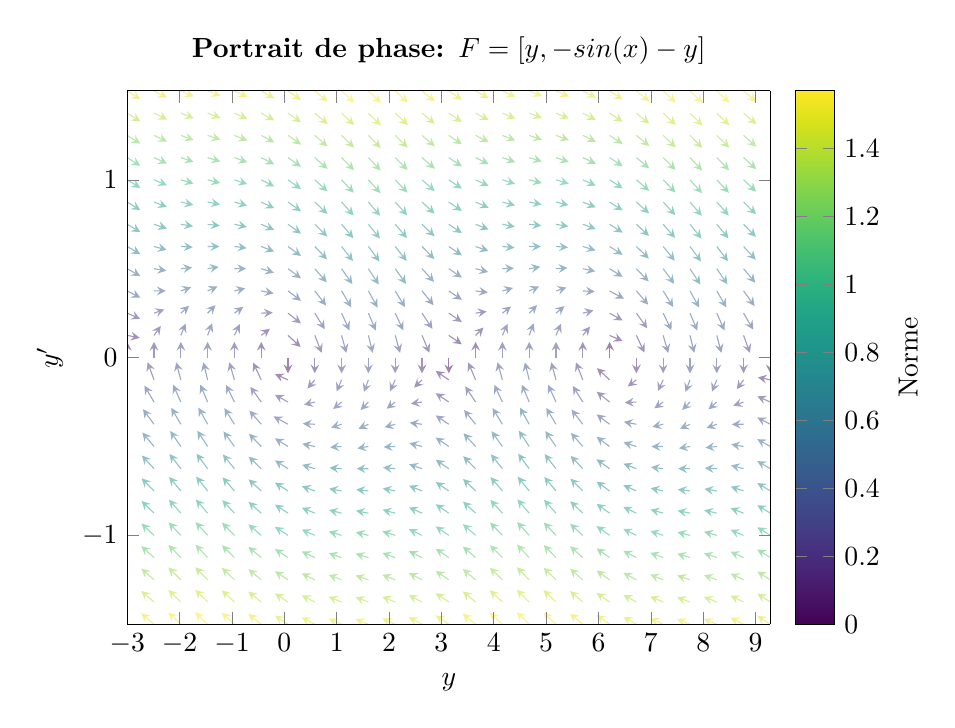
\begin{tikzpicture}
            \tikzset{%
               my arrow/.style={
               postaction={decorate,decoration={
               markings,
               mark=between positions 0.25 and 1 step 0.15 with {\arrow[line width=1.5pt]{stealth}}}}
               }
            }
            \def\xdom{3}
            \def\ydom{1.5}
            \begin{axis}[
               xmin = -\xdom, xmax = \xdom + 2*3.1415,
               ymin = -\ydom, ymax = \ydom,
               zmin = 0, zmax = 1,
               xtick distance = 1,
               ytick distance = 1,
               view = {0}{90},
               scale = 1.25,
               title = {\bf Portrait de phase: $F = [y,-sin(x)-y]$},
               height=7cm,
               xlabel = {$y$},
               ylabel = {$y'$},
               colormap/viridis,
               colorbar,
               colorbar style = {
                  ylabel = {Norme}
               }
            ]
            
            \def\length{sqrt(y^2 + 0.125 * (sin(deg(x)) + 0.2*y)^2)}
               \addplot3[
                  point meta = {\length},
                  quiver = {
                     u = {y/\length},
                     v = {(- 0.125 *(sin(deg(x))) - 0.2*y)/\length},
                     scale arrows = 0.25,
                  },
                  quiver/colored = {mapped color!50},
                  -stealth,
                  domain = -\xdom : \xdom + 2*3.1415 ,
                  domain y = -\ydom : \ydom,
               ] {0};
            \end{axis}
         \end{tikzpicture}
      \end{center}   

